% This thesis template is based on the personal template of Felix Moebius. Thanks, Felix!
% It has been extended and modified by Tobias Pfandzelter at the Scalable Software Systems group of TU Berlin.
% It is licensed under the terms of the MIT license, meaning you are free to use it however you see fit but we accept no liability.
% Good luck writing your thesis!

\documentclass[a4paper, 11pt]{article}

\usepackage[utf8]{inputenc}
\usepackage[T1]{fontenc}
\usepackage{fix-cm}

\usepackage[a4paper, margin=3cm]{geometry}
\usepackage[titletoc, title]{appendix}

\usepackage{color}
\usepackage{booktabs}
\usepackage[all]{nowidow}
\usepackage[dvipsnames]{xcolor}
\usepackage[hidelinks]{hyperref}
\usepackage{acronym}
\usepackage{graphicx}
\usepackage{url}
\usepackage{titlesec}
\usepackage{csquotes}

\usepackage{transparent}
\usepackage{eso-pic}
\usepackage[section]{placeins}
\usepackage{setspace}
\usepackage{parskip}
\usepackage{subcaption}

\renewcommand\thefigure{%
\thesection.\arabic{figure}}
\renewcommand\thesubfigure{%
\thesection.\arabic{figure}.\arabic{subfigure}}
\renewcommand\thetable{%
\thesection.\arabic{table}}

\usepackage[main=english, ngerman]{babel}

% we use the cleveref package to refer to figures, sections, etc.
% instead of "Figure~\ref{fig:example}", write only "\cref{fig:example}" and the word "Figure" (or table, etc) will be inserted normally
\usepackage[noabbrev,capitalise]{cleveref}

\usepackage[
    maxbibnames=99,
    style=alphabetic,
    url=false,
    backend=bibtex8,
    sortcites=true,
]{biblatex}
\bibliography{refs}
\DeclareFieldFormat[online]{urldate}{Last accessed: #1}
\DeclareFieldFormat{eprint}{arXiv: \href{https://arxiv.org/abs/#1}{#1}}
\DeclareFieldFormat[report]{title}{``#1''}


\newcommand{\projectTitle}{Energy-aware Co-location of Scientific Workflow Tasks}
\newcommand{\thesisType}{Master's Thesis}
\newcommand{\authors}{Niklas Fomin}
\newcommand{\matrikel}{464308}
\newcommand{\authorEmail}{\href{mailto:niklas.fomin@campus.tu-berlin.de}{niklas.fomin@campus.tu-berlin.de}}
\newcommand{\examinera}{Prof.~Dr.~habil.~Odej Kao}
\newcommand{\examinerb}{Prof.~Dr. Volker Markl}
\newcommand{\supervisor}{Jonathan Bader}

\newcommand{\projectYear}{2025}
\newcommand{\facultyName}{Fakultät Elektrotechnik und Informatik}
\newcommand{\departmentName}{Fachgebiet Distributed and Operating Systems}

\begin{document}
{\sffamily\color{white}\raggedright\setlength{\parindent}{0cm}\large\onehalfspacing
\AddToShipoutPicture*{
    \put(-4,0){
        \parbox[b][\paperheight]{\paperwidth}{%
            \vfill
            \centering
            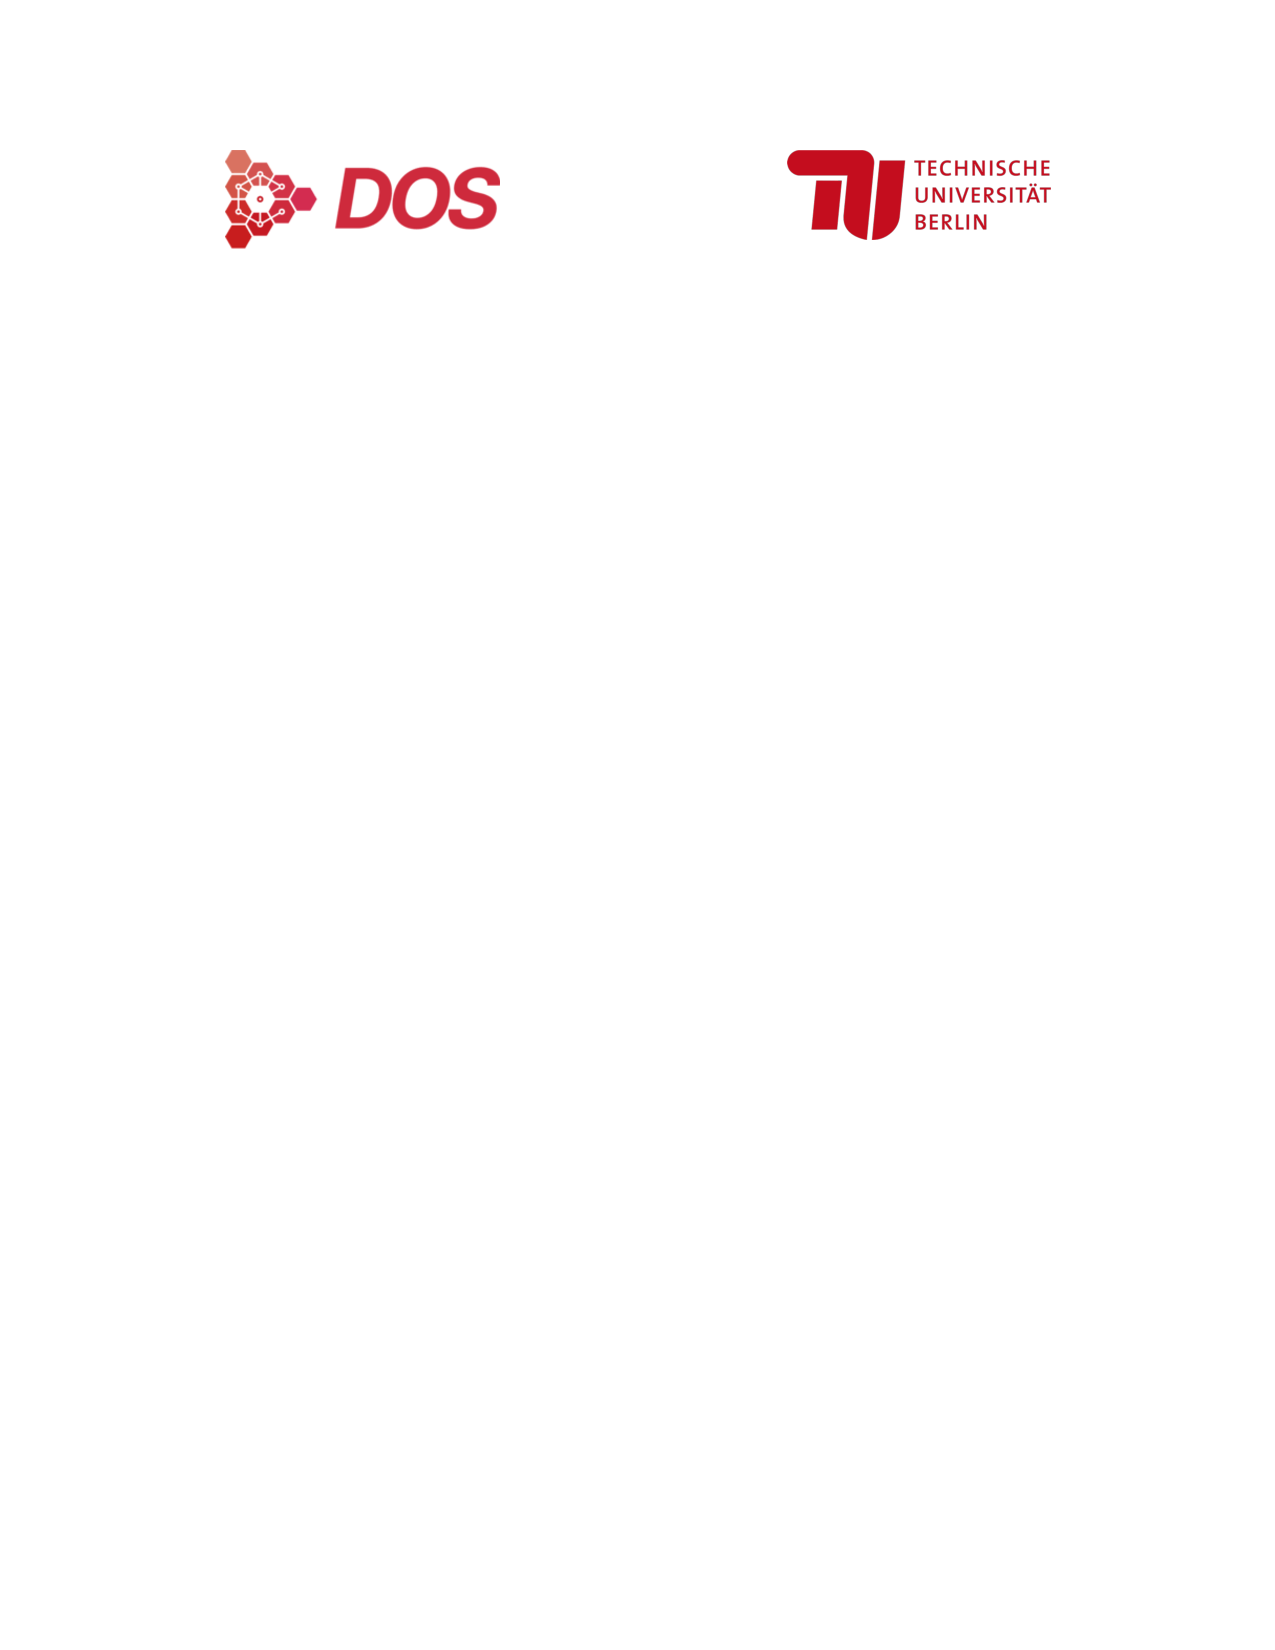
\includegraphics[width=\paperwidth]{title.pdf}%
            \vfill
        }
    }
}

\vfill
\vspace*{5cm}

{\huge\textbf{\projectTitle}\par}
\vspace*{0.5cm}
\textbf{\thesisType}      \\
\vspace*{2cm}
\textbf{Author}               \\
\authors              \\
\matrikel                     \\
\authorEmail                  \\
\vspace*{1cm}
\textbf{Advisor}              \\
\supervisor                   \\
\vspace*{1cm}
\textbf{Examiners}            \\
\examinera                    \\
\examinerb

\vfill

\textbf{Technische Universit\"at Berlin, \projectYear} \\
\small{\facultyName \\
    \departmentName}
\vspace{1cm}
}

\thispagestyle{empty}
\clearpage

\vspace*{\fill}
\begin{centering}
    {\huge\textbf{\projectTitle}\par}
    \vspace{1cm}
    \large{\thesisType}\\
    \vspace{1cm}
    Submitted by:\\
    \authors\\
    \matrikel                     \\
    \authorEmail                  \\
    \vspace{1cm}
    Technische Universit\"at Berlin\\
    \facultyName \\
    \departmentName \\
    \vspace{1cm}
    \projectYear\\

\end{centering}

\vspace*{\fill}
\thispagestyle{empty}
\clearpage

\vspace*{\fill}
{
    % briefly set the footnote to symbols for this disclaimer
    \renewcommand*{\thefootnote}{\fnsymbol{footnote}}
    \noindent
    \begin{otherlanguage}
        {ngerman}
        Hiermit versichere ich, dass ich die vorliegende Arbeit eigenständig ohne Hilfe Dritter und ausschließlich unter Verwendung der aufgeführten Quellen und Hilfsmittel angefertigt habe.
        Alle Stellen die den benutzten Quellen und Hilfsmitteln unverändert oder sinngemäß entnommen sind, habe ich als solche kenntlich gemacht.

        Sofern generische KI-Tools verwendet wurden, habe ich Produktnamen, Hersteller, die jeweils verwendete Softwareversion und die jeweiligen Einsatzzwecke (z.~B.~sprachliche Überprüfung und Verbesserung der Texte, systematische Recherche) benannt.
        Ich verantworte die Auswahl, die Übernahme und sämtliche Ergebnisse des von mir verwendeten KI-generierten Outputs vollumfänglich selbst.

        Die Satzung zur Sicherung guter wissenschaftlicher Praxis an der TU Berlin vom 8. März 2017\footnote{\url{https://www.static.tu.berlin/fileadmin/www/10000060/FSC/Promotion___Habilitation/Dokumente/Grundsaetze_gute_wissenschaftliche_Praxis_2017.pdf}} habe ich zur Kenntnis genommen.

        Ich erkläre weiterhin, dass ich die Arbeit in gleicher oder ähnlicher Form noch keiner anderen Prüfungsbehörde vorgelegt habe.
        \vskip 2cm
        \begin{tabular}{@{}p{.5in}p{4in}@{}}
             & \hrulefill                              \\
             & (Unterschrift) \authors, Berlin, \today \\
        \end{tabular}

    \end{otherlanguage}
    % reset footnote styling for the rest of the thesis
    \renewcommand*{\thefootnote}{\arabic{footnote}}
    \setcounter{footnote}{0}
}

\vspace*{\fill}
\thispagestyle{empty}
\clearpage


\newpage

\section*{Abstract}

FaaS is a cutting-edge new service model that has developed with the current advancement of cloud computing.
It allows software developers to deploy their applications quickly and with needed flexibility and scalability, while keeping infrastructure maintenance requirements very low.
These benefits are very desirable in edge computing, where ever-changing technologies and requirements need to be implemented rapidly and the fluctuation and heterogeneity of service consumers is a considerable factor.
However, edge nodes can often provide only a fraction of the performance of cloud computing infrastructure, which makes running traditional FaaS platforms infeasible.
In this thesis, we present a new approach to FaaS that is designed from the ground up with edge computing and IoT requirements in mind.
To keep it as lightweight as possible, we use CoAP for communication and Docker to allow for isolation between tenants while re-using containers to achieve the best performance.
We also present a proof-of-concept implementation of our design, which we have benchmarked using a custom benchmarking tool, and we compare our results with benchmarks of Lean OpenWhisk, another FaaS platform for the edge.
We find that our platform can outperform Lean OpenWhisk in terms of latency and throughput in all tests but that Lean OpenWhisk has higher success rates for a low number of simultaneous clients.

% GERMAN
\clearpage
\begin{otherlanguage}
    {ngerman}
    \section*{Kurzfassung}
    FaaS ist ein innovatives neues Servicemodell, das sich mit dem aktuellen Vormarsch des Cloud Computing entwickelt hat.
    Softwareentwicklende können ihre Anwendungen schneller und mit der erforderlichen Flexibilität und Skalierbarkeit bereitstellen und gleichzeitig den Wartungsaufwand für die Infrastruktur sehr gering halten.
    Diese Vorteile sind im Edge-Computing sehr wünschenswert, da sich ständig ändernde Technologien und Anforderungen schnell umgesetzt werden müssen und die Fluktuation und Heterogenität der Service-Consumer ein wichtiger Faktor ist.
    Edge-Nodes können jedoch häufig nur einen Bruchteil der Leistung von Cloud-Computing-Infrastruktur bereitstellen, was die Ausführung herkömmlicher FaaS-Plattformen unmöglich macht.
    In dieser Arbeit stellen wir einen neuen Ansatz für FaaS eine Platform vor, die von Grund auf unter Berücksichtigung von Edge-Computing- und IoT-Anforderungen entwickelt wurde.
    Um den Overhead so gering wie möglich zu halten, nutzen wir CoAP als Messaging-Protokoll und Docker, um Applikationen voneinander zu isolieren, während Container wiederverwendet werden, um die bestmögliche Leistung zu erzielen.
    Wir präsentieren auch eine Proof-of-Concept-Implementierung unseres Designs, die wir mit einem eigenen Benchmarking-Tool getestet haben, und vergleichen unsere Ergebnisse mit Benchmarks von Lean OpenWhisk, einer weiteren FaaS-Plattform für die Edge.
    Wir stellen fest, dass unsere Plattform Lean OpenWhisk in Bezug auf Latenz und Durchsatz in allen Tests übertreffen kann, Lean OpenWhisk jedoch höhere Erfolgsraten bei einer geringen Anzahl gleichzeitiger Clients aufweist.
    \cite{10.1007/978-3-030-30143-9_15}
\end{otherlanguage}

\clearpage

\tableofcontents

\section{Introduction}
\label{cha:introduction}

% Data Center Graph, then bridge gap to HPC and Scientific Workflows,Mention that a lot was done in HPC Co-Scheduling and also with the co-scheduling paradigm in cloud computing or interfernce with latency-sensitive jobs but not very much with co-location strategies themselves. Make a nice example of such a problem and how it looks like and why it can be beneficial.
\subsection{Problem Motivation \& Description}
\label{subse:problem_motivation_description}
% Section 1: Start with my graph and the initial problem
The rapid growth in data center power consumption has emerged as a pressing societal issue. As of March 2024, global statistics report more than 9,000 operational data centers worldwide, with this number continuing to rise steadily. Consequently, total annual energy consumption across data centers has been roughly doubling every four years with some now reaching capacities of up to 500 MW, comparable to the electricity demand of a city of one million residents. With the rapid growth in data volumes and processing requirements over the last two decades, workflow applications have grown in complexity, while computing infrastructures have advanced in processing capacity and workload management capabilities \cite{Coleman_2021}.
High-performance computing (HPC) refers to the pursuit of maximizing computational capabilities through advanced technologies, methodologies, and applications, enabling the solution of complex scientific and societal problems [citation]. HPC data centers consist of large numbers of interconnected compute and storage nodes, often numbering in the thousands, and rely on job schedulers to allocate resources, manage queues, and monitor execution. While these infrastructures provide the backbone for highly demanding applications, their intensive power draw does not only arise from computation but also from networking, cooling, and auxiliary equipment and makes them major consumers of electricity and significant contributors to climate change \cite{Silva_2024}.

% Figure
\begin{figure}[H]
    \centering
    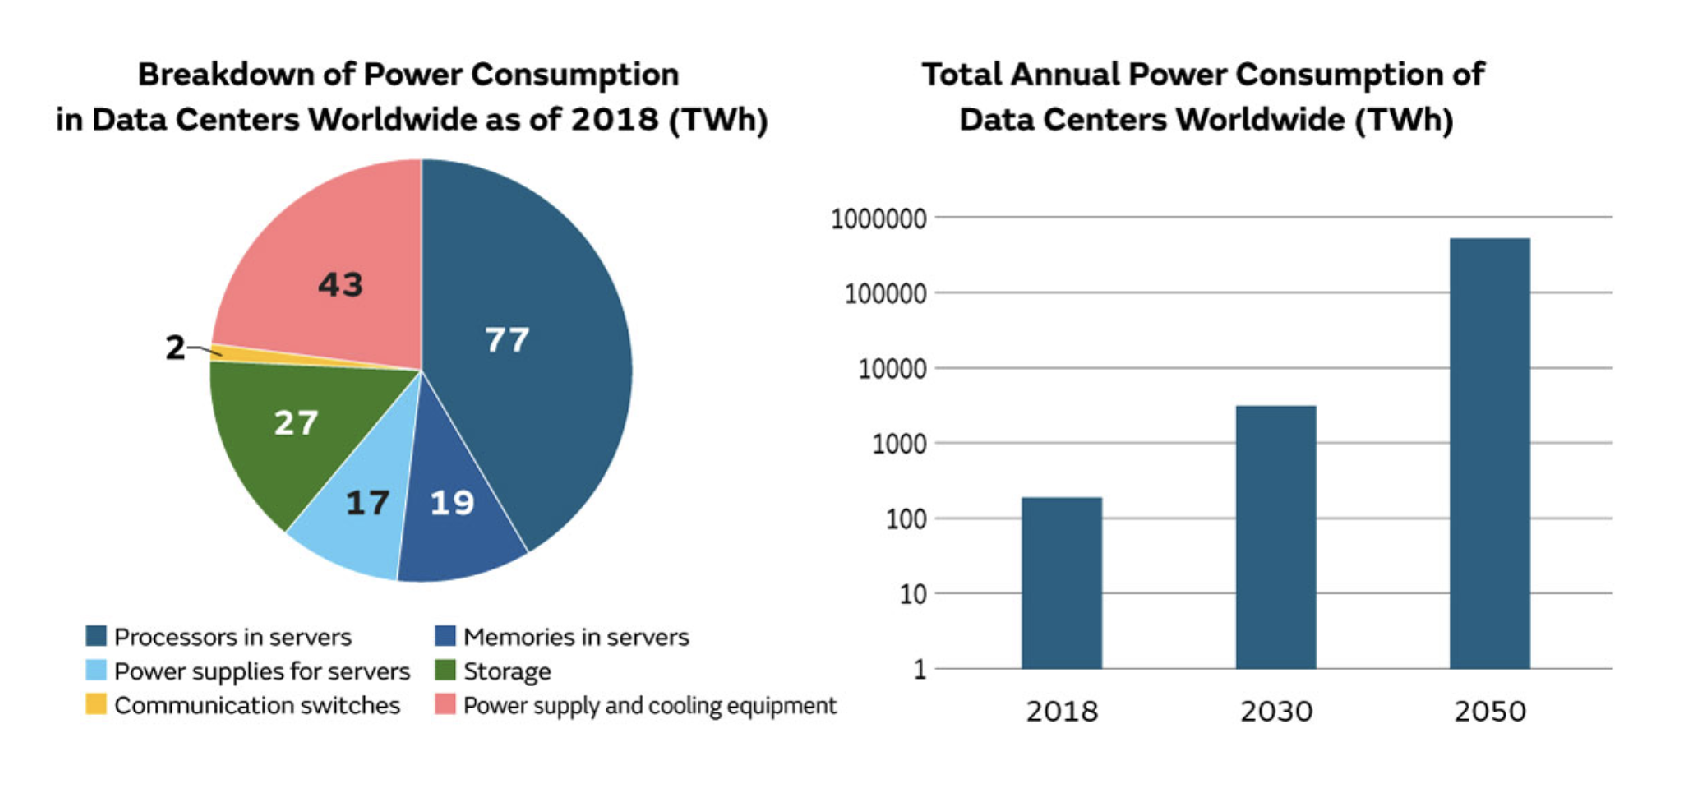
\includegraphics[scale=0.5]{fig/01/01-motivation.pdf}
    \small
    \caption{Breakdown of power consumption in data centers}
    \label{fig:01-motivation}
    \tiny
    Breakdown of power consumption in data centers and future outlook for power consumption.
\end{figure}

% Section 2: Move on to HPC and Workflows
A key driver of this trend is the exponential growth in data collection, storage, and processing across scientific disciplines. Scientific Workflow Management Systems (SWMSs) have become essential tools for managing this complexity, enabling researchers to exploit computing clusters for large-scale data analysis in domains such as remote sensing, astronomy, and bioinformatics. However, workflows executed through SWMSs are often long-running, resource-intensive, and computationally demanding, which translates into high energy consumption and substantial greenhouse gas emissions. Nevertheless, practitioners face challenges in assessing which approaches for mitigation are most applicable, effective with concerns to multiple objectives \cite{thamsen2025energyawareworkflowexecutionoverview}.
One central objective that this work focuses on is grounded in the challenge that tasks within data-driven workflows often appear in multiple instances and may vary substantially depending on input data, parameters, or execution environments their patterns in resource demand, energy consumption, and carbon emissions fluctuate during runtime rather than remaining constant.
This work primarily focuses on an aspect of workflow research that has received limited attention: modeling and managing the co-location of parallel tasks in containers and virtual machines.
To address this challenge, we apply continuous monitoring to enable fine-grained, time-dependent task models that accurately capture resource usage patterns. The central objective of this work is to leverage knowledge of task behavior to enhance the co-location process—the intermediate stage between task-to-machine mapping and scheduling—where decisions are made about which tasks should share compute resources to balance performance and energy efficiency.
While related concepts have been explored in the context of co-scheduling at the operating system level or in cloud environments where batch jobs run alongside latency-critical services, the online co-location problem addressed here differs. In our setting, decisions about which tasks to execute together on the same virtual machine must be made dynamically at each scheduling interval, requiring continuous adaptation to the current workflow state and resource conditions. The importance of such decisions can be illustrated through an example by \cite{inproceedings}. Consider two compute-bound programs (A1, A2) and two memory-bound programs (B1, B2) to be co-scheduled across two nodes. If both compute-bound tasks share one node while both memory-bound tasks share the other, the memory-intensive programs will heavily compete for bandwidth, causing severe slowdowns and doubling their execution time. In contrast, pairing each compute-bound task with a memory-bound one allows both to utilize different resources efficiently, resulting in no slowdown at all. This demonstrates two fundamental principles of co-location: tasks that heavily use the same resource should not be co-located, and complementary resource usage—such as pairing CPU-intensive and memory-intensive workloads—can maximize system performance.
Furthermore, previous studies have shown that effective co-scheduling of this kind can significantly enhance both energy efficiency and system throughput in high-performance computing environments. In the best cases, runtime can be reduced by up to 28\% and total energy consumption by approximately 12\% compared to isolated, dedicated execution. However, the extent of improvement depends strongly on the diversity and ratio of jobs in the scheduling queue \cite{7349920}. To address this, we propose a hierarchical clustering approach that groups tasks by dissimilarity to encourage complementary co-location. This mechanism is integrated into a workflow simulation framework, where several scheduling algorithms are implemented to demonstrate how informed, runtime co-location decisions can enhance task mapping and overall workflow efficiency.

% TODO: make cursive
These challenges motivate the central goal of this work: modelling the complementary co-location of scientific workflow tasks using fine-grained, time-dependent resource usage profiles and embedding it into workflow execution for energy and performance aware decision making during runtime.

\subsection{Research Question \& Core Contributions}
\label{subse:research_question_core_contributions}

The central questions this thesis seeks to address are:

\begin{enumerate}[label=\textbf{RQ}\arabic*]
    \item How can fine-grained, time-dependent models of workflow tasks be developed to capture fluctuating patterns of computational resource usage and energy consumption during execution?
    \item How can the co-location of workflow tasks be modeled so that their interference is minimized and the resulting shared usage of resources leads to lower overall energy consumption and carbon emissions while performance is maintained?
    \item How can co-location models and time-dependent task characterizations be integrated into resource management systems and workflow scheduling frameworks to enable adaptive, energy-aware execution at scale?
\end{enumerate}

% TODO: Add footnote for nf-core repo
The resulting core contributions of this thesis are:
\begin{itemize}
    \item The implementation of a monitoring client, capable of serving the relevant monitoring layers for scientific workflow execution which collects fine-grained, time-dependent resource usage data for workflow tasks during execution that was used for low-level data collection on 9 nf-core pipelines.
    \item The design and further development of a novel online task co-location approach that utilizes time series data to compute for any given set of tasks clusters with complementary resource usage patterns.
    \item The development of a simulator that integrates the proposed co-location approach into the workflow execution phase.
    \item The conceptual implementation of a scheduler, able to predict the performance and energy consumption of co-located tasks using two machine learning models.
    \item The evaluation of the co-location approach in simulation using 9 nf-core workflows, demonstrating its effectiveness in reducing energy consumption while maintaining performance.
\end{itemize}
\subsection{Structure of the Thesis}
\label{subse:structure_of_the_thesis}
The remainder of this thesis is structured as follows: Chapter \ref{cha:background} presents the fundamentals of this work, covering performance monitoring, scientific workflow systems, the co-location problem, cluster resource management and machine learning. Chapter \ref{cha:relatedwork} introduces related work within the domain of optimizing Scientifc Workflow execution and objectives in line with these of this work. Furthermore, Chapter \ref{cha:approach} depicts the approach to the problem in both a theoretical and practical manner and ultimately defines the realization of the approach. The corresponding implementation is elaborated in Chapter \ref{cha:implementation}. Moreover, Chapter \ref{cha:evaluation} evaluates the steps conducted to achieve the implementation of the overall approach using both empirical data and a simulation environment. Chapter \ref{cha:discussion} interprets the key findings and discusses some limitations of this work. Finally, Chapter 8 concludes this thesis and gives an outlook on the impact of this work for the future.

\clearpage
\section{Background}
\label{cha:background}

This chapter provides the necessary background for the thesis. Section 2.1 introduces the domain of High-Performance Computing (HPC), with a focus on modern computational hardware (2.1.1) and virtualization technologies (2.1.2). Section 2.2 then discusses scientific workflows as a representative HPC application, beginning with a definition of scientific workflows (2.2.1), followed by their management systems (2.2.2), and concluding with workflow tasks as their smallest management unit (2.2.3). Section 2.3 introduces the domain of energy-aware computing, while Section 2.4 addresses workflow monitoring, including monitoring targets (2.4.1), resource monitoring (2.4.2), energy monitoring (2.4.3), and task characterization using monitoring data (2.4.4). Section 2.5 presents the co-location problem, which constitutes the core of this thesis. It motivates the problem through resource contention (2.5.1), discusses its relationship to workflow scheduling and task mapping (2.5.2), and provides a general overview with the guiding boundaries that shape the definition of workflow task co-location used throughout this work. Section 2.6 introduces the role of machine learning in scientific workflow processing, focusing on its application in resource management (2.6.1) and the theoretical background of the models applied in this thesis. This includes Kernel Canonical Correlation Analysis (KCCA) (2.6.2.1), Random Forest Regression (2.6.2.2), Linear Regression (2.6.2.3), and Agglomerative Clustering for task clustering (2.6.2.4). Finally, Section 2.7 outlines the evaluation methodology, with an emphasis on simulation approaches and a description of the WRENCH framework for simulating distributed computing environments (2.7.1).

\subsection{High Performance Computing}
\label{sec:background_hpc}
% TODO: Include citation HPC book, Chapter 1.1
High-Performance Computing (HPC) encompasses a collection of interrelated disciplines that together aim to maximize computational capability at the limits of current technology, methodology, and application. At its core, HPC relies on specialized electronic digital machines, commonly referred to as supercomputers, to execute a wide variety of computational problems or workloads at the highest possible speed. The process of running such workloads on supercomputers is often called supercomputing and is synonymous with HPC. The fundamental purpose of HPC is to address questions that cannot be adequately solved through theory, empiricism, or conventional commercial computing systems. The scope of problems tackled by supercomputers extends beyond traditional scientific and engineering applications to include challenges in socioeconomics, the natural sciences, large-scale data management, and machine learning. An HPC application refers both to the problem being solved and to the body of code, or ordered instructions, that define its computational solution.

What distinguishes HPC systems from conventional computers is their organization, interconnectivity, and scale. Here, scale refers to the degree of both physical and logical parallelism: the replication of essential physical components such as processors and memory banks, and the partitioning of tasks into units that can be executed simultaneously. While parallelism exists in consumer devices like laptops with multicore processors, HPC systems exploit it on a vastly larger scale, structured across multiple hierarchical levels. Their supporting software is designed to orchestrate and manage operations at this level of complexity, ensuring efficient execution across thousands of interconnected components.

\subsubsubsection{Modern HPC Hardware}
\label{sec:background_hpc_hardware}
% Include graphic inspired from Chapter 1.1, page 7 of HPC book.
High performance computer architecture determines how very fast computers are formed and function. High performance computing (HPC) architecture is not specifically about the lowest-level technologies and circuit design, but is heavily influenced by them and how they can be most effectively employed in supercomputers. HPC architecture is the organization and functionality of its constituent components and the logical instruction set architecture (ISA) it presents to computer programs that run on supercomputers. HPC architecture exploits its enabling technologies to minimize time to solution, maximize throughput of operation, and serve the class of computations associated with large, usually numeric-intensive, applications. In recent years supercomputers have been applied to data-intensive problems as well, popularly referred to as “big data” or “graph analytics”. For either class of high-end applications, HPC architecture is created to overcome the principal sources of performance degradation, including starvation, latency, overheads, and delays due to contention. It must facilitate reliability and minimize energy consumption within the scope of performance and data requirements. Cost is also a factor, affecting market size and ultimate value to domain scientists and other user communities. Finally, architecture shares in combination with the many other layers of the total HPC system the need to make application programming by end users as easy as possible.

HPC system performance depends on the speed of its components, with processor clock rate being a key factor. A major challenge arises from mismatches in cycle times across technologies, such as fast processor cores versus much slower DRAM. To bridge this gap, modern architectures use memory hierarchies that combine high-capacity DRAM with faster SRAM caches. Performance is also shaped by communication speed, measured in bandwidth and latency, which vary with technology and distance. Ultimately, HPC architecture seeks to balance computation, memory, and communication speeds while optimizing cost, power, and usability to maximize application performance.
Efficiency in HPC refers to how effectively system components are utilized when executing a workload. A common metric is floating-point efficiency, defined as the ratio of sustained floating-point performance to the theoretical peak, both measured in FLOPs. While once meaningful in an era when floating-point operations were costly, this measure has become less representative as data movement and memory access now dominate in terms of time, energy, and die space. Nevertheless, FLOP-based efficiency remains the most widely reported measure.

Power consumption is a critical factor in HPC, as processors, memory, interconnects, and I/O devices all require electricity, and the resulting heat must be removed to avoid failure. Processor sockets alone may consume 80–200 W, and cooling adds significant overhead, sometimes exceeding 20\% of total power use. Air cooling suffices for smaller systems, but high-density, high-performance systems increasingly rely on liquid cooling to achieve higher packing density and performance. Modern processors further support power management through dynamic voltage and frequency scaling, variable core activation, and thermal monitoring. These mechanisms enable a balance between power consumption and performance, guided by software that can set or adjust configurations at runtime based on workload demands.

The multiprocessor class of parallel computer represents the dominant architecture in contemporary supercomputing. Broadly defined, it consists of multiple independent processors, each with its own instruction control, interconnected through a communication network and coordinated to execute a single workload. Three main configurations of multiprocessor systems exist: symmetric multiprocessors (SMPs), massively parallel processors (MPPs), and commodity clusters. The distinction lies in memory organization. SMPs use a shared memory model accessible by all processors, MPPs assign private memory to each processor, and cluster-based designs combine both approaches by grouping processors into nodes that share memory locally while maintaining separation across nodes. Modern multicore systems often follow this hybrid structure, balancing performance, scalability, and complexity.
% TODO: Maybe include graphic that shows overview

A shared-memory multiprocessor consists of multiple processors with direct hardware access to a common main memory. This architecture allows any processor to read or write data produced by another, requiring an interconnection network that ensures cache coherence across all processors. Cache coherence guarantees correctness by keeping local caches consistent, often implemented through protocols such as MESI, where writes are detected and other caches are updated or invalidated accordingly.

Shared-memory multiprocessors are commonly divided into two categories based on memory access times. In symmetric multiprocessors (SMPs), all processors can access any memory block in equal time, known as uniform memory access (UMA). While contention for memory banks can still cause delays, the system provides equal opportunity to all processors. SMPs are widely used in enterprise servers, workstations, and multicore laptops, and often serve as nodes within larger parallel systems.

Nonuniform memory access (NUMA) architectures extend shared-memory designs by allowing all processors to access the full memory space but with different access times depending on locality. NUMA leverages fast local memory channels alongside slower global interconnects, enabling greater scalability than SMPs. However, this places additional responsibility on software developers to optimize data placement in order to achieve high performance. NUMA systems emerged in the late 20th century and remain a key design for scaling shared-memory multiprocessors.

% TODO: Add NUMA graphic
% TODO: Add AMD stuff

\subsubsection{Virtualization in HPC}
\label{sec:background_hpc_virtualization}
% TODO: Cite paper: Survey on Virtualization of HPC, M. Shao IEEE
With the growing demand for High-Performance Computing (HPC), hardware resources have continued to expand in scale and complexity, with increasingly intricate interconnections between system components. A central challenge lies in maximizing both performance and resource utilization. Virtualization technologies offer a means to improve resource utilization in HPC environments, but often at the cost of performance overhead. Multi-user usage scenarios, combined with the stringent performance requirements of HPC workloads, place high demands on virtualization approaches. Furthermore, the highly customized nature of HPC systems complicates the integration of virtualization solutions. This work examines operating system-level and application-level virtualization within HPC, outlines the current limitations, and discusses potential directions for future developments.

Virtualization at the operating system level has been widely explored through technologies such as VMware, Xen, LXC, and KVM, each offering different trade-offs between usability, security, and performance. VMware, one of the earliest and most established solutions, allows multiple operating systems to run simultaneously on a single host, offering strong isolation, security, and ease of configuration. However, the performance overhead introduced by full virtual machines is too high for HPC workloads, which demand near-native computational speed. Xen, developed as an open-source virtual machine monitor, improved performance compared to VMware but required operating system modifications, making it less developer-friendly and leading to reduced long-term adoption. More recent solutions such as LXC and KVM integrate virtualization more closely with the Linux kernel, reducing overhead compared to traditional VMs. While these operating system–level containers are lighter than VMware or Xen, they still introduce performance penalties, with KVM in particular showing unacceptable overhead for CPU-intensive HPC applications. Moreover, KVM requires hardware-level virtualization support, limiting its applicability.

In multi-tenant HPC environments, the dynamic sharing of hardware resources introduces complex power–performance relationships, as concurrently executed tasks exhibit varying levels of power consumption across different resources. Users increasingly expect the flexibility of cloud-like environments, where execution conditions resemble their native setups without significant performance loss. Container-based HPC environments address this demand by isolating groups of processes into separate applications that run densely on available hardware threads. \cite{Kuity_2023}.

Virtualization enables the provisioning of resources to multiple users on the same physical machine with the goal of maximizing utilization. Depending on the abstraction layer, different virtualization technologies provide distinct benefits. Containers, which virtualize at the operating system level, offer lightweight isolation and have become widely adopted for deploying microservices. They effectively bridge the gap between development and production by supporting continuous integration and deployment pipelines.
Containers leverage the host operating system kernel and typically incur far less management and runtime overhead compared to virtual machines. Prior studies have shown that container performance often approaches native execution, particularly for CPU- and memory-intensive workloads, whereas VMs tend to suffer greater degradation for memory, disk, and network-intensive applications. In comparative analyses, Docker containers have demonstrated near-native efficiency for CPU and memory tasks but exhibit performance bottlenecks in certain networking and storage configurations. Research has also highlighted scalability challenges, including increased startup times as the number of containers grows, as well as interference effects when multiple containers share disk- or network-intensive workloads on the same host. These findings underline the fact that performance in containerized environments is strongly dependent on workload characteristics and resource contention patterns. Despite advances such as workload-aware brokering systems aimed at improving energy efficiency and utilization, limited attention has been paid to how workload nature and interference influence consolidation decisions \cite{8397647}.

% TODO: Cite paper: Survey on Virtualization of HPC, M. Shao IEEE
Application-level virtualization operates above the kernel layer, sharing both the kernel and underlying hardware. This approach is most prominently represented by containers, with Docker introducing a transformative model of packaging and deployment. By encapsulating application dependencies into images and leveraging ecosystems such as Docker Hub, Docker enables rapid and portable application deployment. However, in HPC environments, Docker raises serious concerns. Security risks emerge from its daemon-based execution model, which runs with root privileges, and its resource allocation mechanism conflicts with HPC scheduling managers like Slurm, PBS, or SGE. These schedulers typically rely on cgroups to enforce job-level resource limits, but such constraints are ineffective when bypassed by Docker’s daemon. Furthermore, Docker lacks robust support for MPI and multi-node collaboration, making it unsuitable for large-scale HPC workloads.

% TODO: Cite paper: Survey on Virtualization of HPC, M. Shao IEEE
To address these issues, container solutions such as Singularity and Shifter were developed specifically with HPC requirements in mind. Singularity allows users to build and test applications in local environments and then deploy them seamlessly on HPC systems. Unlike Docker, it does not rely on a persistent daemon, thus resolving security and resource management concerns. Singularity also supports multiple container image formats, including compatibility with Docker images, and integrates efficiently with HPC resource managers. Its design ensures that containers incur minimal overhead, as virtualization occurs only at the application level with a shared kernel, making it particularly well-suited for HPC contexts where performance efficiency is critical.

% TODO: Containerization graphic
% TODO: Virtual Machine graphic

\subsection{Scientific Workflows}
\label{sec:background_workflows}

% TODO: Include more stuff from 
% \cite{Scientific worflows: past, present and future}
\subsubsection{Scientific Workflow Management Systems}
\label{sec:background_workflows_swms}
Scientific Workflow Management Systems (SWMSs) enable the composition of complex workflow applications by connecting individual data processing tasks. These tasks, often treated as black boxes, can represent arbitrary programs whose internal logic is abstracted away from the workflow system. The resulting workflows are typically modeled as directed acyclic graphs (DAGs), where channels define the dependencies between tasks: the output of one task serves as the input for one or more downstream tasks. This abstraction allows users to design scalable, reproducible workflows while managing execution complexity across diverse computational environments \cite{thamsen2025energyawareworkflowexecutionoverview}.

Scientific Workflow Management Systems (SWMSs) provide a simplified interface for specifying input and output data, enabling domain scientists to integrate and reuse existing scripts and applications without rewriting code or engaging with complex big data APIs. This abstraction lowers the entry barrier for developing and executing large-scale workflows. In parallel, cloud computing has become an increasingly popular execution environment, complementing or replacing traditional HPC clusters. Clouds offer advantages such as elastic scalability, flexible pay-as-you-go pricing models, and access to a wide range of heterogeneous hardware resources, making them attractive for diverse workflow workloads \cite{Bader_2022}.

% TODO: Add graphic of SWMS architecture in general

\subsubsection{Examples of Scientific Workflows}
\label{sec:background_workflows_examples}
% TODO: Add graphic of pipeline 
Scientific workflows are compositions of sequential and con- current data processing tasks, whose order is determined by data interdependencies [4]. A task is the basic data process- ing component of a scientific workflow, consuming data from input files or previous tasks and producing data for follow- up tasks or output files (see Figure 1). A scientific workflow is usually specified in the form of a directed, acyclic graph (DAG), in which individual tasks are represented as nodes. Scientific workflows exist at different levels of abstraction: abstract, concrete, and physical. An abstract workflow mod- els data flow as a concatenation of conceptual processing steps. Assigning actual methods to abstract tasks results in a concrete workflow. If this mapping is performed auto- matically, it is called workflow planning [5]. To execute a concrete workflow, input data and processing tasks have to be assigned to physical compute resources. In the context of scientific workflows, this assignment is called scheduling and results in a physical and executable workflow [6]. Low-level batch scripts are a typical example of physical workflows \cite{Bux2013}.

% TODO: Add section about HPC and Scientific Workflows with reference to earlier section
\subsubsection{Scientific Workflow Tasks}
\label{sec:background_workflows_examples}
Workflow applications are typically executed per input, or per set of related inputs, enabling coarse-grained data parallelism at the application level. Multiple tasks can run concurrently if independent inputs are processed by the same workflow, and parallelism also arises within a single input when workflow graphs fork, allowing downstream tasks to execute simultaneously. Conversely, many workflows begin with parallel execution of different tasks whose outputs are later joined, synchronizing multiple workflow paths.

Due to their complexity and scale, workflows often consist of large numbers of tasks with multiple parallel paths and are executed on clusters—collections of interconnected compute nodes managed as a single system. Scientific Workflow Management Systems (SWMSs) submit ready-to-run tasks to cluster resource managers such as Slurm or Kubernetes, which allocate resources according to user-defined requirements like CPU cores and memory. Task communication is typically implemented via persistent cluster storage systems (e.g., Ceph, HDFS, or NFS), where intermediate data is written and read between tasks. This approach ensures flexible scheduling, fault tolerance through restartable intermediate states, and simplified execution management.

While SWMSs usually treat tasks as black boxes, opening these tasks for optimization can significantly improve performance. In particular, adapting code to the available hardware, such as optimizing for specific CPUs or accelerators, can reduce runtime. Since certain code segments disproportionately affect overall task execution time, focusing on these hotspots offers an effective strategy for workflow-level performance improvement \cite{thamsen2025energyawareworkflowexecutionoverview}.

% TODO: Add graphic of task 
% TODO: Mention task disclaimer for writing ease


\subsection{Energy-Aware Computing}
\label{sec:background_energyawarecomputing}
% TODO: Include more examples of the relevancy of energy-aware computing
\cite{thamsen2025energyawareworkflowexecutionoverview}
Power consumption in computing systems can broadly be divided into static and dynamic components. Static power is drawn even when components are idle, often reaching up to half of peak power, while dynamic power depends on utilization and increases with workload. This inefficiency has motivated the concept of energy-proportional computing, in which energy use per operation scales directly with utilization. Hardware trends and techniques such as Dynamic Voltage and Frequency Scaling (DVFS) have improved proportionality, while workload consolidation further increases efficiency by concentrating tasks on fewer resources.

Beyond compute, data centers also consume energy for cooling, lighting, and auxiliary operations. This is measured by Power Usage Effectiveness (PUE), which expresses the ratio between total data center energy use and the share consumed by IT equipment. While leading hyperscale centers achieve PUE values close to 1.1, the global average remains higher, and the metric has known limitations, including sensitivity to workload characteristics and the inability to capture whole-system trade-offs.

The climate impact of energy use further depends on carbon intensity, i.e., the emissions associated with each unit of consumed electricity. This varies geographically and temporally with the mix of fossil, nuclear, and renewable generation sources. As such, carbon intensity can fluctuate substantially over hours and regions, meaning that both location and timing of computation influence emissions.

Breaking down component-level energy use, CPUs typically dominate server consumption, accounting for 40–66\% of total power, with significant static and dynamic contributions. Memory is the second largest consumer, drawing a smaller but relatively stable share, while storage devices show limited dynamic variation and modest overall consumption. Networking equipment consumes comparatively little, with low dynamic variation, though attributing its energy use to specific workloads is non-trivial.

A geoscience workflow (FORCE) was executed on a commodity cluster using 21 nodes for 315 minutes to process 304 GB of satellite images. The hardware setup led to an estimated operational energy use of 15.8 kWh, factoring in average data center overhead (PUE 1.61). Given Germany’s 2021 grid carbon intensity of 439 gCO₂e/kWh, this corresponds to about 6.95 kgCO₂e emissions per run, or 20.8 kgCO₂e for the three repetitions used to report median results—roughly equal to driving 53 miles in a gasoline car. Beyond operational emissions, the embodied carbon footprint of the hardware was considered. With an estimated 1200 kgCO₂e per node over its lifetime and 0.00599\% of lifetime usage during the experiment, the workflow’s share amounts to about 1.5 kgCO₂e per run, or 4.5 kgCO₂e for three executions. Thus, both operational and embodied emissions contribute to the total footprint of the workflow evaluation.

\subsection{Monitoring Scientific Workflows}
\label{sec:background_monitoring}

\subsubsection{Performance Monitoring}
\label{sec:background_monitoring_performance}
% TODO: Insert citation for HPC Book
Performance monitoring is a critical stage in application development, extending beyond functional correctness and validation of results. Even after thorough testing with diverse datasets and computational modes, hidden inefficiencies may remain that limit the application’s ability to fully exploit the underlying hardware. This is especially significant in parallel computing, where inefficiencies are amplified across many processor cores, leading not only to longer runtimes but also to higher computational costs, as users are often charged proportionally to aggregate machine time. Monitoring helps ensure that performance is not degraded by preventable factors, for example by checking whether computation times match processor capabilities or whether communication delays align with message sizes and network bandwidth. Instrumentation of code segments can provide such insights, though even basic measurements introduce latency and overhead that may distort results or even alter execution flow. To reduce this, statistical sampling is often employed, recording snapshots of program state at intervals rather than logging every event. Sampling periods can be tuned to balance accuracy against intrusiveness. Hardware-based approaches offer another alternative: modern CPUs provide dedicated performance counters for events such as instruction retirement, cache misses, or branches. These counters operate transparently, incurring virtually no overhead, though they are limited to a predefined set of measurable events. Together, these techniques form the basis of effective performance monitoring, allowing developers to identify and address bottlenecks without unduly interfering with execution.

\subsubsection{Monitoring Layers}
\label{sec:background_monitoring_layers}
While low-level tools can provide detailed insights into system resource usage, linking these measurements to higher-level abstractions such as workflow tasks remains challenging. In large-scale scientific workflows executed on distributed environments like clusters or clouds, tasks may be scheduled on arbitrary nodes and may even share resources with other tasks. As a result, locally observed traces of CPU, memory, or I/O usage cannot be directly attributed to specific tasks. To bridge this gap, resource usage profiles from compute nodes must be correlated with metadata such as workflow logs or job orchestrator information (e.g., container management data). Establishing this information chain enables the classification of observed behavior at the task level, highlighting inefficient or resource-intensive components of the workflow that offer the greatest potential for optimization.

Existing monitoring frameworks focus primarily on processes or systems and generally lack the ability to map resource usage back to workflow tasks, especially in multi-tenant or distributed environments. This limits the ability to isolate the contribution of individual tasks to overall resource consumption. Moreover, metrics natively provided by workflow management systems are often coarse-grained, capturing only summary statistics for task lifetimes. To obtain fine-grained insights into task-level behavior, additional instrumentation and mapping strategies are required to connect low-level monitoring data with workflow abstractions \cite{Witzke2024}.

% TODO: Insert adapted graphic of monitoring layers, inspired by Bader.
The proposed architectural blueprint for workflow monitoring is structured into four layers: the resource manager, the workflow, the machine, and the task layer. These layers represent logical distinctions within a scientific workflow execution environment, each focusing on a different monitoring subject and retrieving metrics from lower layers as needed. Unlike user-centric designs, this approach emphasizes system components rather than interaction flows. Higher layers provide increasingly abstract views, relying only on selected metrics from underlying layers while, in theory, being able to access all. For instance, at the resource manager level, systems such as Slurm, Kubernetes, or HTCondor only require aggregate metrics like task resource consumption or available machine resources, without depending on fine-grained traces such as syscalls. The workflow layer captures metrics tied to the workflow specification, while the machine layer delivers detailed reports of node-level resource usage. At the lowest level, the task layer focuses on fine-grained task execution metrics. Together, this hierarchy balances abstraction and granularity, ensuring that relevant monitoring information is exposed at the appropriate level to support both workflow execution and performance optimization \cite{Bader_2022}.

The monitoring architecture is structured into four interdependent layers that capture different levels of abstraction within a workflow execution environment. At the top, the resource manager layer supervises the cluster, orchestrates task assignments, and provides coarse-grained monitoring. It contributes aggregated information such as active workflows, running and queued tasks, node health status, and distributed file system states. To enable correct task placement, it draws on workflow-level identifiers and DAG structures, machine-level metrics like available cores or memory, and task-level resource usage and execution status. The workflow layer refines this view by capturing execution semantics, such as dependencies between tasks expressed as DAGs, workflow progress, runtime statistics, makespan, and error reports. The machine layer focuses on per-node monitoring, reporting both general metrics (e.g., CPU and memory utilization) and fine-grained hardware characteristics such as architecture, clock rates, disk partitions, and virtualization context. At the lowest level, the task layer provides the most detailed insights, including logs, execution times, time-series resource usage, and kernel-level traces such as system calls or I/O activity. These fine-grained metrics are essential for diagnosing failures and identifying performance bottlenecks. Together, the four layers form a hierarchical structure where higher layers abstract and summarize information from lower ones, enabling a comprehensive and scalable approach to workflow monitoring \cite{Bader_2022}.

Scientific workflow management systems (SWMSs) provide varying degrees of built-in monitoring support, which is often complemented by external tools. Pegasus integrates tightly with HTCondor as its resource manager and submits monitoring data directly into a relational database, enabling real-time querying and visualization with external tools such as ElasticSearch or Grafana. Nextflow, originally developed for bioinformatics workflows, has since expanded into other domains and produces monitoring reports once workflow executions are complete. Airflow, with its strong integration into Python, exports selected metrics to StatsD, from where they can be forwarded to systems such as Prometheus for monitoring. Snakemake, also Python-based, supports report generation after execution and offers live monitoring through its Panoptes service, which streams data to an external server accessible via API. Argo, designed natively for Kubernetes, provides a web-based interface where users can access reports and logs of previous executions alongside live monitoring features. Despite these capabilities, most resource managers do not natively handle workflow-level submissions. Consequently, SWMSs typically manage task dependencies and submit tasks sequentially as their requirements are satisfied, with notable exceptions such as HTCondor’s DAGMan meta-scheduler and Slurm’s built-in dependency mechanisms \cite{Bader_2022}.

\subsubsection{Resource Monitoring}
\label{sec:background_monitoring_resource}
% TODO: Insert citation for ebpf book
Monitoring scientific workflows requires tools that can capture and relate information across different components of a computing system, since no single perspective provides sufficient detail for effective optimization. Low-level system monitors can reveal CPU, memory, or I/O usage but lack awareness of which workflow tasks generate that load, while workflow management systems expose task-level metrics that are often too coarse to identify inefficiencies. Similarly, resource managers like Slurm or Kubernetes aggregate machine usage but obscure fine-grained behavior. To close these gaps, specialized tools must be employed at each system layer—resource manager, workflow, machine, and task—and their outputs correlated. This layered approach ensures that high-level abstractions such as workflows can be linked to detailed system traces, allowing bottlenecks to be identified, failures diagnosed, and task placements optimized with respect to both performance and energy consumption. Without combining tools across layers, monitoring remains fragmented, leaving critical inefficiencies hidden in complex, distributed execution environments. In the following, we briefly discuss tools and approaches for monitoring each of these layers in detail while section % reference to section approach for monitoring
will go into much more detail.

Building on the need for layered monitoring, it is essential to introduce some fundamental terms and techniques that describe how monitoring data is collected and analyzed across system components. Central among these is tracing, which captures fine-grained event-based records such as system calls, I/O operations, or network packets. Tracing provides detailed raw data, often with high volume, that can either be post-processed into summaries or analyzed on the fly using programmatic tracers such as those enabled by the Berkeley Packet Filter (BPF). BPF allows small programs to run directly in the kernel, making it possible to process events in real time and reduce the overhead of storing and analyzing massive trace logs. In contrast, sampling tools collect subsets of data at regular intervals to create coarse-grained performance profiles. While sampling introduces less overhead than tracing, it provides only partial insights and can miss important events. Together with fixed hardware or software counters, tracing and sampling form the backbone of observability—the practice of understanding system behavior through passive observation rather than active benchmarking. Observability thus provides the conceptual umbrella under which monitoring tools operate, ranging from low-level system probes to workflow-aware abstractions. 
The BPF ecosystem provides several user-friendly front ends for tracing, most notably BCC (BPF Compiler Collection) and bpftrace. BCC was the first higher-level framework, offering C-based kernel programming support alongside Python, Lua, and C++ interfaces, and it introduced the libbcc and libbpf libraries that remain central to BPF instrumentation. It also provides a large collection of ready-to-use tools for performance analysis and troubleshooting. bpftrace, in contrast, offers a concise, domain-specific language that makes it well suited for one-liners and short custom scripts, while BCC is better for complex programs and daemons. A lighter-weight option, ply, is also being developed for embedded Linux environments. These frameworks, maintained under the Linux Foundation’s IO Visor project, collectively form what is often referred to as the BPF tracing ecosystem.These distinctions are crucial, as they shape how different tools are applied at the task, machine, workflow, and resource manager layers, and they form the basis for the more concrete monitoring techniques discussed in the following sections.

% TODO: Insert overview graph with monitoring targets on OS-level

Building on this, monitoring CPU usage fundamentally relies on understanding how time is distributed across these execution modes and how the scheduler allocates processor resources among competing tasks. Metrics such as user time, system time, and idle time provide the basis for identifying imbalances, while additional indicators like context switches, interrupt handling, and run queue lengths reveal how efficiently the scheduler manages concurrency. Since background kernel activities and hardware interrupts can consume significant CPU cycles outside of explicit user processes, distinguishing their contribution is essential for accurate analysis. Together, these metrics allow researchers and practitioners to detect inefficiencies such as excessive kernel overhead, overloaded cores, or unfair task distribution—insights that are critical when analyzing the performance of scientific workflows running on shared or large-scale computing infrastructures. A practical strategy for CPU performance analysis begins with verifying that a workload is running and truly CPU-bound, which can be confirmed through utilization metrics and run queue latency. Once established, usage should be quantified across processes, modes, and CPUs to identify hotspots such as excessive system time or uneven load distribution. Additional steps include measuring time spent in interrupts, exploring hardware performance counters like instructions per cycle (IPC), and using specialized BPF tools for deeper insights into stalls, cache behavior, or kernel overhead. This structured approach helps progressively narrow down the root causes of performance issues.
In close relation to CPU monitoring, effective memory performance analysis requires tracking how memory behavior influences compute efficiency. Since CPUs frequently stall waiting for data, metrics such as page faults, cache misses, and swap activity can directly translate into wasted cycles. A systematic strategy begins with checking whether the out-of-memory (OOM) killer has been invoked, as this signals critical memory pressure. From there, swap usage and I/O activity should be examined, since heavy swapping almost always leads to severe slowdowns. System-wide free memory and cache usage provide a high-level view of available resources, while per-process metrics help identify applications with excessive resident set sizes (RSS). Monitoring page fault rates and correlating stack traces can reveal which tasks or files drive memory pressure, while tracing allocation calls such as brk() and mmap() offers a complementary perspective on memory growth. At the hardware level, performance counters measuring cache misses and memory accesses give insights into where CPUs are stalling on memory I/O. Together, these monitoring steps build a detailed picture of how memory usage interacts with CPU performance, helping to uncover bottlenecks and inefficiencies that limit overall throughput.

Following CPU and memory, file system monitoring should focus on workload behavior at the logical I/O layer and its interaction with caches and the underlying devices. Key signals include operation mix and rates (reads, writes, opens/closes, metadata ops such as rename/unlink), latency distributions for I/O (including tails), and the balance of synchronous versus asynchronous writes. Cache effectiveness is central: track page-cache hit ratios over time, read-ahead usefulness (sequential vs random access), volumes of dirty pages and write-back activity, and directory/inode cache hit/miss rates. Attribute I/O to files and processes to spot hot files and short-lived file churn, and examine I/O size distributions to detect pathologically small requests. Relate logical I/O to physical I/O to assess whether caching is working or the workload is spilling to disk; include error rates and filesystem-specific events (e.g., journaling) for completeness. Finally, watch capacity and fragmentation risk (very high fill levels), mount options that affect performance semantics (e.g., atime, sync modes), and any lock contention visible in the file system path. A compact table or time-series dashboard for these metrics is helpful for diagnosis and comparison across workloads [cite].

In storage subsystems, background monitoring should characterize I/O where it matters for delivered performance and capacity planning rather than enumerate specific tools. At minimum, track request latency as a distribution (including tails) and decompose it into time queued in the operating system versus service time at the device; sustained high queue time indicates saturation regardless of nominal utilization. Measure throughput and IOPS per device together with queue depth to relate load to response, and record I/O size histograms and access locality (sequential vs. random) to explain latency modes. Distinguish operation classes—reads vs. writes, synchronous vs. asynchronous, metadata, readahead, flush/discard—since policies and devices handle them differently and they can interfere (e.g., reads stalling behind large write bursts). Attribute I/O to processes/containers and, where applicable, to workflow tasks so that noisy neighbors and hot spots can be isolated. Track error and timeout rates at the device interface to separate performance issues from reliability faults. Contextual signals such as filesystem cache hit ratio (logical vs. physical I/O), write-back pressure, and device fill level complement block-layer metrics and help explain shifts in latency or throughput. Segment all measurements per device and scheduling policy, and analyze them over time to identify persistent contention, bimodal behavior, and regressions that warrant tuning, task remapping, or rescheduling.

Containers are a lightweight virtualization technology that isolate applications while sharing the same host operating system kernel. Their implementation in Linux builds on two core mechanisms: namespaces, which provide isolation by restricting the view of system resources such as processes, file systems, and networks; and control groups (cgroups), which regulate resource usage, including CPU, memory, and I/O. Container runtimes such as Docker or orchestration frameworks like Kubernetes configure and combine these mechanisms to provide isolated execution environments. Two versions of cgroups exist in the kernel. Version 1 is still widely used in production systems, while version 2 addresses several shortcomings, including inconsistent hierarchies and limited composability, and is expected to become the default for containerized workloads in the near future.

From a performance monitoring perspective, containers introduce challenges that extend beyond those encountered in traditional multi-application systems. First, cgroups may impose software limits on CPU, memory, or disk usage that can constrain workloads before physical hardware limits are reached. Detecting such throttling requires monitoring metrics that are not visible through standard process- or system-wide tools. Second, containers can suffer from resource contention in multi-tenant environments, where “noisy neighbors” consume disproportionate shares of the available resources, leading to unpredictable performance degradation for co-located containers. This is particularly critical in Kubernetes deployments, where hundreds of containers may share a host and rely on fair scheduling enforced by the kernel and the container runtime.

A further complication lies in attribution. The Linux kernel itself does not assign a global container identifier. Instead, containers are represented as a combination of namespaces and cgroups, which complicates mapping low-level kernel events back to the higher-level abstraction of a specific container. While some workarounds exist—such as deriving identifiers from PID or network namespaces, or from cgroup paths—this mapping is non-trivial and runtime-specific. Consequently, many traditional monitoring tools remain container-unaware, often reporting host-level metrics even when executed inside containers. This mismatch can obscure important performance characteristics, such as CPU scheduling delays or memory pressure within a specific container, and may hinder the diagnosis of resource bottlenecks.

To address these issues, container monitoring must operate at multiple levels of abstraction. Metrics must capture both coarse-grained resource usage across cgroups and fine-grained kernel events such as scheduling latencies, memory allocation faults, and block I/O delays. At the same time, the collected data needs to be attributed correctly to the corresponding container environment in order to identify interference, diagnose bottlenecks, and evaluate orchestration policies. These requirements have motivated the use of extended monitoring techniques such as Berkeley Packet Filter (BPF) tracing, which can instrument kernel paths at runtime and associate low-level events with container-related constructs such as namespaces and cgroups.

Hypervisors enable hardware virtualization by abstracting physical resources and presenting them as fully isolated virtual machines, each running its own kernel. Two common configurations exist: bare-metal hypervisors, such as Xen, which schedule guest virtual CPUs directly on physical processors, and host-based hypervisors, such as KVM, which rely on a host kernel for scheduling. Both models often involve additional I/O handling layers, for example QEMU, which introduce latency but can be optimized through techniques such as shared memory transports and paravirtualized device drivers. Over time, virtualization efficiency has improved significantly with processor extensions like Intel VT-x and AMD-V, paravirtualization interfaces for hypercalls, and device-level virtualization (e.g., SR-IOV). Modern platforms, such as AWS Nitro, minimize software overhead by offloading core hypervisor functionality to dedicated hardware components.

Monitoring hypervisors poses challenges similar to containers but with a different focus. Since each VM runs its own kernel, guest-level monitoring tools can operate normally, but they cannot always observe the virtualization overheads introduced by the hypervisor. Key concerns include the frequency and latency of hypercalls in paravirtualized environments, the impact of hypervisor callbacks on application scheduling, and the amount of stolen CPU time—periods when a guest’s vCPU is preempted by the hypervisor. From the host perspective, additional events such as VM exits provide insight into how often guests trigger traps to the hypervisor, for example on I/O instructions or privileged operations, and how long these exits last. Attribution is further complicated because exit reasons vary widely across workloads and hypervisor implementations.

Effective analysis therefore requires combining guest-side monitoring of virtualized resources with host-side tracing of hypervisor interactions. Guest instrumentation can measure hypercall behavior, detect high callback overheads, or quantify CPU steal time, while host tracing can expose exit patterns, QEMU-induced I/O delays, and hypervisor scheduling effects. As with containers, BPF-based tracing has become particularly valuable in this domain, since it can capture low-level kernel events with high resolution, linking them to hypervisor operations. With the shift toward hardware-assisted virtualization, fewer hypervisor-specific events remain visible to the guest, making host-level tracing and cross-layer correlation increasingly central to performance monitoring of virtualized environments.

\subsubsection{Monitoring Energy Consumption}
\label{sec:background_monitoring_energy}
Energy monitoring of servers combines hardware-aware measurement with system-level attribution to quantify operational emissions and guide optimizations. At its core is a decomposition of power into static (idle) and dynamic (utilization-dependent) components; modern platforms aim for energy-proportional behavior via DVFS and workload consolidation, yet static draw can still be a large fraction of peak power. Component contributions vary—CPUs frequently dominate (tens to ~150 W per socket depending on model and load), memory adds a steadier baseline (few watts per 8 GB, modest dynamic range), storage ranges from low-swing HDDs to more energy-proportional SSDs, and network switches exhibit very low dynamic variability—so monitoring must separate baseline from incremental use. Measurements should be translated into environmental impact using facility Power Usage Effectiveness (PUE) and grid carbon intensity (CI), acknowledging that CI varies by region and time. Practically, on-node electrical telemetry is obtained from Intel RAPL via MSRs and OS interfaces (powercap, perf events), with user-space polling or eBPF-assisted collection; higher-level tools (e.g., CodeCarbon, PowerAPI, Scaphandre) build on these to attribute energy to processes. For multi-tenant hosts, thread/container-level attribution benefits from correlating RAPL energy with performance counters across context switches (e.g., BPF-based approaches such as DEEP-mon), enabling per-thread, per-container, and per-host aggregation with negligible overhead. A robust methodology therefore (i) establishes the static baseline and a CPU model (e.g., ACPS/frequency-aware) to avoid double counting, (ii) profiles disks and NICs under controlled I/O sizes/rates while flushing caches and subtracting baseline+CPU, and (iii) scales results through PUE and CI for carbon accounting, yielding repeatable, architecture-agnostic estimates suitable for power-aware scheduling, capping, and capacity planning.
% TODO: Cite doctoral thesis on RAPL
% TODO: Include schematic overview from doctoral thesis, Figure 1.1, 2.3 and 2.4
% Also mention that this is not a substantial part of the thesis but it rather builds on that
Improving the energy efficiency of high-performance computing (HPC) and data center systems requires accurate and fine-grained monitoring of power consumption at the level of individual servers and their components. Traditional approaches based on external wattmeters or hardware sensors are costly, intrusive, and often lack the accuracy and granularity required for detailed analysis, particularly in heterogeneous and highly dynamic workloads. This has motivated the adoption of hardware-assisted mechanisms such as Intel’s Running Average Power Limit (RAPL), which since the Sandy Bridge architecture has provided direct, low-overhead measurements of energy consumption across CPU cores, the processor package, DRAM, and sometimes integrated GPUs. RAPL enables real-time power monitoring that can be integrated into scheduling, optimization, and power modeling frameworks, offering a practical alternative to coarse external meters or performance-counter-based estimation models. While RAPL has been widely used due to its accuracy, availability, and negligible overhead, its limitations in granularity and the interpretation of certain domains remain open research challenges. In HPC environments, where maximizing performance per watt is critical, RAPL has become a central tool for attributing energy costs to workloads, profiling applications, and guiding energy-aware scheduling, but ongoing work is needed to refine its role in comprehensive system-level energy modeling and management.

Beyond general breakdowns of server energy consumption, the focus in high-performance computing has shifted towards how to obtain accurate and fine-grained measurements without relying on costly or intrusive external hardware. Traditional approaches such as wattmeters or chassis-level sensors remain valuable for coarse measurements, but they lack the granularity to attribute consumption to individual subsystems or workloads. Performance monitoring counters and operating system statistics have therefore been increasingly combined with modeling techniques to approximate component-level power use, though such models often struggle with accuracy under fluctuating workloads. This has motivated the adoption of hardware-integrated interfaces, most notably Intel’s Running Average Power Limit (RAPL), which provides direct access to energy consumption data for CPU packages, cores, and memory domains. In contrast to external metering, RAPL enables low-overhead, programmatic, and high-resolution measurements, making it a widely used foundation for power modeling and energy-aware scheduling in HPC systems.

The Running Average Power Limit (RAPL) interface, first introduced with Intel’s Sandy Bridge architecture, provides a hardware-based mechanism to both measure and limit energy consumption across different CPU domains. Its primary purpose is twofold: offering fine-grained, high-frequency energy measurements and enabling power capping to manage thermal output. RAPL exposes several power domains depending on the processor generation, such as the processor package (PKG), which accounts for the entire socket including cores and uncore components, PP0 for cores, PP1 for integrated GPUs, DRAM for attached memory, and PSys in newer architectures like Skylake for system-level monitoring of the SoC. Among these, the PKG domain is universally available, while support for others varies across server and desktop models. Each domain provides cumulative energy consumption values via model-specific registers (MSRs), updated at millisecond resolution and expressed in architecture-specific energy units. These values can be accessed directly through the MSR driver in Linux or via higher-level interfaces such as sysfs, perf, or the PAPI library, offering flexibility in integrating RAPL into monitoring and profiling workflows. With its combination of accuracy, low overhead, and broad accessibility, RAPL has become a central mechanism for energy measurement and modeling in high-performance and data center computing.
% Include RAPL schema, but mention drawbacks due to AMD architecture

% End with deep-mon and also mention other tools that will be discussed later in the approach/implementation section
With the increasing adoption of containerization in both cloud and HPC environments, fine-grained energy attribution has become a crucial requirement for efficient workload management. While Intel’s RAPL interface provides accurate measurements of CPU and memory energy consumption at high granularity, its integration into container-level monitoring fills an important gap left by earlier VM- and node-centric approaches. Scientific workflows, which often run as complex pipelines of heterogeneous tasks within containers, particularly benefit from this capability, as it enables precise accounting of energy usage per workflow component. This allows power-aware schedulers and orchestrators to balance performance and energy efficiency, identify hotspots, and optimize resource allocation across distributed systems. Tools such as DEEP-mon build on RAPL by combining kernel-level event tracing with container-level aggregation, offering low-overhead monitoring that can attribute energy costs down to threads and containers. Such capabilities are essential to advance sustainable HPC by enabling detailed profiling of workflow execution and supporting energy-aware scheduling decisions in containerized infrastructures.


\subsection{The Co-location Problem}
\label{sec:background_colocation}
% Begin with the origin of co-location being in operting systems scheduling
% Mention that there are many levels of co-location as in FONDA, VMs, containers and in resource managers
% TODO: Cite Barry Linnerts slides from OS or find the direct source
The problem of scientific workflow task co-location can be traced back to classical operating system scheduling, where the core challenge lies in allocating activities to functional units in both time and space. Traditionally, scheduling in operating systems refers to assigning processes or threads to processors, but this problem appears at multiple levels of granularity, from whole programs to fine-grained instruction streams executed within superscalar architectures. On multiprocessor and multicore systems, the scheduler must not only decide when to run a task but also where, since shared caches, memory bandwidth, and execution units create interdependencies between colocated workloads. Early work in operating systems introduced coscheduling or gang scheduling, where groups of related tasks are executed simultaneously to reduce synchronization delays, exploit data locality, and minimize contention for shared resources. These concepts are directly relevant to modern scientific workflows, where multiple interdependent tasks are often colocated on the same nodes or cores in high-performance computing environments. The performance and energy efficiency of workflows are therefore closely tied to scheduling decisions, as co-located tasks may either benefit from shared resource usage or suffer from interference, making scheduling a fundamental problem for efficient workflow execution.
In high-performance computing (HPC), task co-location poses unique challenges due to the complex interplay of shared resources in modern multi-core architectures. Processors share on-chip structures such as last-level caches, memory controllers, and interconnects, as well as off-chip memory bandwidth, creating significant opportunities for contention when multiple applications run concurrently. This contention can result in severe performance degradation, making it critical to understand and predict the impact of co-location on application efficiency. A naïve approach of exhaustively profiling all potential co-locations is infeasible in practice, given the enormous number of possible workload combinations. Instead, research has focused on predictive methodologies that use application-level indicators, such as cache usage or memory access patterns, to estimate interference effects. This has led to classification schemes that characterize applications both by their sensitivity to co-located workloads and by their capacity to disrupt others. 
Building on the challenges of co-location in multi-core systems, the problem becomes even more pronounced when considering scientific workflows, which consist of heterogeneous tasks with highly variable and dynamic resource requirements. Assigning each task to a separate server leads to poor energy efficiency, as servers continue to draw a substantial fraction of their peak power even under low utilization. Server consolidation thus emerges as a promising strategy, where multiple workflow tasks are mapped onto fewer servers to reduce total power consumption and resource costs. In this context, the terms consolidation and co-location can be used interchangeably, as both refer to the placement of multiple tasks onto the same physical resources with the aim of improving efficiency. However, consolidation is far from trivial: the resource usage of colocated tasks is not additive, and interference effects can significantly impact both power consumption and application performance. Furthermore, the temporal variation in workflow task demands requires runtime-aware provisioning strategies to avoid resource contention and performance degradation. These complexities underline the need for methodologies that can accurately predict and manage co-location trade-offs, paving the way for addressing the specific challenges of scientific workflow task consolidation in HPC and cloud environments \cite{5644899}

\subsubsection{Resource Contention and Interference}
\label{sec:background_colocation_interference}
% Distiniguish a little bit between node-level contention and core-contention, but put the methods to the related work section and wove into the approach part as the reasoning for the design decisions.
% TODO: Make a sketch based on Terrible Twins Paper Figure 1
The fundamental motivation for addressing co-location in HPC and cloud environments lies in the problem of resource contention. When processes execute on different cores of the same server, they inevitably share hardware resources such as caches, buses, memory, and storage. This sharing often leads to interference, slowing down execution compared to scenarios where tasks have exclusive access to these resources. In extreme cases, memory traffic contention has been shown to cause super-linear slowdowns, where execution times more than double, making sequential execution more efficient than poorly chosen co-schedules. For large-scale systems hosting thousands of tasks, this contention complicates job scheduling, as schedulers must avoid placing workloads that compete heavily for the same resources. Without accurate estimates of resource usage or slowdown potential, scheduling decisions risk becoming guesswork, reducing overall efficiency. Importantly, poor scheduling is not limited to high-resource applications: even pairing computationally bound tasks that do not interfere can be suboptimal if it prevents beneficial co-scheduling with memory-bound applications. This highlights that effective co-location must avoid both high-contention pairings and missed opportunities for complementary workload placement. Addressing these challenges requires systematic strategies that recognize and mitigate interference, providing the key motivation for studying co-location in the context of scientific workflow tasks \cite{inproceedings}.

In HPC environments, where users submit batch jobs to multi-core compute nodes, efficient resource utilization is critical for balancing throughput, makespan, and job duration. However, parallel applications often fail to fully exploit all allocated cores due to bottlenecks in shared resources such as memory or I/O bandwidth, leading to inefficiencies and longer runtimes. Co-allocating multiple applications on the same nodes has been explored as a strategy to reduce makespan and improve overall system throughput, yet it remains uncommon in production systems because contention for shared resources like last-level caches or memory controllers can increase individual job durations. One approach to mitigate these drawbacks is process mapping, where processes of parallel applications are carefully assigned to specific cores to minimize communication costs and interference. With the growing complexity of HPC architectures, featuring deep memory hierarchies and high core densities, process mapping has become increasingly important. Still, existing solutions often focus solely on single-application performance and rely on costly profiling runs, limiting their applicability in co-located, real-world production workloads. This creates a clear need for methodologies that can address co-location and mapping challenges jointly, enabling more efficient use of HPC resources without sacrificing fairness or performance \cite{10.1007/978-3-031-48803-0_31}.


\subsubsection{Scientific Workflow Scheduling \& Task Mapping}
\label{sec:background_colocation_scheduling}
In this section, we describe two widely-used energy-aware workflow scheduling algorithms that leverage the traditional power consumption model for making scheduling decisions described in the previous section. We then evaluate the energy consumption for schedules computed by these two algorithms using both the traditional and the realistic models. We do so by using a simulator that can simulate the power consumption of a workflow execution on a compute platform for either model. We perform these simulations based on real-world execution traces of three I/O-intensive workflow applications. The specific scheduling problem that these algorithms aim to solve is as follows.
Scheduling Problem Statement. Consider a workflow that consist of single-threaded tasks. This workflow must be executed on a cloud platform that comprises homogeneous, multi-core compute nodes. Initially, all compute nodes are powered off. A compute node can be powered on at any time. Virtual machine (VM) instances can be created at any time on a node that is powered on. Each VM instance is started for an integral number of hours. After this time expires, the VM is shutdown. A node is automatically powered off if it is not running any VM instance. The cores on a node are never oversubscribed (i.e., a node runs at most as many VM instances as it has cores). A VM runs a single workflow task at a time, which runs uninterrupted from its start until its completion. The metrics to minimize are the workflow execution time, or makespan, and the total energy consumption of the workflow execution \cite{HosseiniShirvani2024}.

n this section, we select several representative scheduling algorithms from each category per their performance and impact. Based on the scheduling approaches, we introduce four types of scheduling algorithms:
Task-based (scheduling task-by-task): In the literature, they are also called list-based scheduling. In these algorithms, tasks are ordered based on some priority ranking and then a scheduling decision is made for each task in that order. Path-based (scheduling path-by-path): In these algorithms, a workflow is partitioned into paths based on some criteria and then a scheduling decision is made for each path.
BoT-based (scheduling BoT-by-BoT): In these algorithms, a workflow is partitioned into BoTs (Bag of Tasks) such that each BoT is a set of tasks that have no data dependencies among them, and a scheduling decision is made for each BoT.
Workflow-based (scheduling workflow-by-workflow): In these algorithms, all tasks in a workflow are simultaneously scheduled and then the schedule for each task is improved using some procedure to improve the quality of the global workflow schedule \cite{a survery}.

Node-level and core-level co-location represent two distinct layers of contention within HPC systems. At the node level, tasks share off-chip resources such as memory bandwidth, network interfaces, and I/O subsystems, where heavy communication or I/O-intensive jobs can interfere with one another and degrade performance. At the core level, co-located tasks contend for on-chip resources like private and shared caches, pipelines, and execution units, which can lead to latency, cache thrashing, or reduced instruction throughput. These co-location challenges differ fundamentally from scheduling and task mapping: scheduling determines when tasks execute and mapping decides on which resource they run, while co-location focuses on how tasks interact when placed together on the same hardware. Even though all three may share the objective of improving throughput and minimizing energy consumption, co-location directly addresses the resource interference between tasks and therefore requires strategies that go beyond scheduling order or resource assignment. The challenge lies in predicting and managing these interference effects so that consolidation for energy savings does not undermine overall performance, which makes co-location a critical but separate consideration within workflow execution strategies.
The co-location problem in scientific workflow execution arises directly from the heterogeneous ways tasks can currently be placed on HPC and cloud infrastructures. Tasks may be co-located on the same physical node, executed exclusively on a node, distributed across multiple nodes inside containers, or deployed in virtual machines where either one task runs per VM or multiple VMs are consolidated onto the same host. Each of these deployment choices introduces different levels of contention: cores may compete for shared last-level caches, memory bandwidth, or interconnect capacity, while nodes may compete for I/O channels, network interfaces, or access to distributed storage. Because workflows are executed in these diverse environments, the challenge of co-location becomes embedded into scheduling and task mapping decisions—not as a separate process, but as a cross-cutting concern that determines how efficiently tasks can share resources without incurring performance degradation or excessive energy costs.
% TODO: Make a cool schema about co-location, task mapping and scheduling that showcases a couple of scenarios, motivates them and then shows the focus of this work
% Also bring up the correlation between contention and energy efficiency and make reference to the approach section.
In the context of scientific workflows, the relation between resource contention and energy efficiency becomes particularly critical, as under-utilized or poorly consolidated resources can lead to significant power waste. Since servers consume a large fraction of their peak power even at low utilization, mapping each workflow task to a separate node often results in inefficiency. Consolidating tasks onto fewer servers can mitigate this by increasing utilization and reducing overall energy consumption. However, consolidation also raises the challenge of interference, as colocated tasks may contend over CPU, memory, disk, or network resources, potentially degrading performance and offsetting the energy savings. This trade-off highlights why the task co-location problem cannot be ignored: energy-efficient workflow execution requires balancing resource consolidation to reduce idle power draw with careful awareness of contention patterns to avoid excessive slowdowns. In this sense, energy efficiency and performance are inherently tied to how tasks are colocated, making it essential to embed power-awareness into workflow scheduling and mapping strategies \cite{5644899} \cite{Lee2012}.

\subsection{Machine Learning in Scientific Workflow Computing}
\label{sec:background_ml}


\subsubsection{Intelligent Resource Management}
\label{sec:background_ml_resourcemanagement}
% TODO: Intro sentence on resource managers in scientific workflows
While traditional HPC systems often avoid colocating applications on the same node due to unpredictable interference effects, the potential benefits of improved throughput and energy efficiency make the problem worth revisiting. When colocated tasks are bottlenecked by different resources, resource utilization can be increased without altering application code, opening opportunities for more efficient execution. Machine learning offers a promising avenue to address the complexity of this problem, as it can capture non-trivial relationships between hardware performance monitoring counters and the resulting performance degradation under colocation. Unlike rule-based heuristics, machine learning models can generalize across diverse applications and workloads, enabling predictive insights into slowdown and contention effects. Although training and inference may be computationally demanding, practical optimizations have shown that machine learning can be applied with manageable overhead, making it a viable tool to guide scheduling and task placement decisions for scientific workflows in HPC environments. Resource colocation in multi-core HPC systems inherently introduces contention for shared on- and off-chip resources such as caches, memory controllers, and interconnects, which can significantly affect application performance. Traditional heuristic-based scheduling approaches, for example those relying only on LLC miss rates, have shown limited success as they often fail to capture the complex and non-linear slowdown effects caused by colocated applications. To overcome these limitations, recent research has turned to machine learning techniques that exploit performance monitoring counters (PMCs) to predict degradation effects more accurately. By training models offline on representative workloads and deploying them in scheduling decisions at runtime, such approaches enable degradation-aware colocation strategies that minimize makespan and improve resource utilization. This integration of predictive modeling into workload management represents a significant step towards intelligent, energy-efficient execution of HPC workloads, where scheduling decisions are not only resource-aware but also contention-sensitive, directly addressing the challenges posed by colocating diverse scientific applications \cite{ZACARIAS2021125}.

When executing scientific workflows on large-scale computing infrastructures, researchers are required to define task-level resource limits, such as execution time or memory usage, to ensure that tasks complete successfully under the control of cluster resource managers. However, these estimates are often inaccurate, as resource demands can vary significantly across workflow tasks and between different input datasets, leading either to task failures when limits are underestimated or to inefficient overprovisioning when limits are set too conservatively. Overprovisioning, while preventing failures, reduces cluster parallelism and throughput, as excess resources are reserved but left unused, while incorrect runtime estimates can distort scheduling decisions and degrade overall system efficiency. To address this, recent research has explored workflow task performance prediction as a means to automate the estimation of runtime, memory, and other resource needs. Machine learning plays a central role in these efforts, with approaches ranging from offline models trained on historical execution data, to online models that adapt dynamically during workflow execution, to profiling-based methods applied before execution. Performance prediction models can integrate into both workflow management systems and resource managers, enabling more informed scheduling, efficient resource utilization, and improved energy- and cost-aware computing. This establishes task-level performance prediction as a crucial foundation for advancing scientific workflow execution towards higher reliability, efficiency, and sustainability \cite{bader2025predictingperformancescientificworkflows}.

\subsubsection{Utilized Machine Learning Algorithms in this Thesis}
\label{sec:background_ml_algorithms}
% Summary sentence about what models are used and what for and where else in the thesis it will be more elaborated on them.

\paragraph{Linear Regression}
\label{sec:background_ml_lr}
% TODO: Add formal example notation and add citation for sklearn documentation.
Linear regression is a fundamental statistical method used to model the relationship between one or more explanatory variables and a continuous response variable. It estimates coefficients by minimizing the residual sum of squares, providing an optimal linear fit between predictors and outcomes. The model assumes linearity, independence of errors, homoscedasticity, and normally distributed residuals. Ordinary Least Squares (OLS) is the most common approach, where the coefficients are computed analytically from the design matrix. However, when predictors are highly correlated, multicollinearity can occur, making the coefficient estimates unstable and sensitive to noise in the data. Despite this limitation, linear regression remains widely used due to its interpretability, computational efficiency, and ability to serve as a baseline for more complex regression techniques.

\paragraph{Kernel Canonical Correlation Analysis}
\label{sec:background_ml_kcca}
% TODO: Add formal example notation and maybe some graphs from cca zoo that show something.
% Add example
Canonical Correlation Analysis (CCA) is a statistical technique designed to identify and maximize correlations between two sets of variables. Unlike Principal Component Analysis, which focuses on variance within a single dataset, CCA aims to find linear projections of two datasets such that their correlation is maximized. The result is a set of canonical variables that capture the strongest relationships between the two domains. Kernel Canonical Correlation Analysis (KCCA) extends this idea by applying kernel methods, allowing the detection of nonlinear relationships. In KCCA, the data are implicitly mapped into high-dimensional feature spaces through kernel functions, and correlations are then maximized in that transformed space. This enables KCCA to capture more complex dependencies than linear CCA, making it particularly powerful in settings where relationships between datasets are not strictly linear \cite{1202783}.
Kernel Canonical Correlation Analysis (KCCA) works by taking kernel matrices of two datasets and solving a generalized eigenvalue problem to identify projections that are maximally correlated. Intuitively, this means that KCCA maps both datasets into high-dimensional feature spaces defined by kernel functions and then finds directions in these spaces where the correlation between the two datasets is strongest. In practice, one dataset can represent resource usage metrics while the other represents performance or power measurements. KCCA then identifies correlated structures—such as clusters of similar usage patterns and their corresponding performance or energy behaviors—revealing how variations in resource usage align with variations in system-level outcomes. This makes KCCA particularly suitable for analyzing complex, nonlinear relationships in workflow execution, where resource usage and energy efficiency are intertwined \cite{5644899}.
Ensemble methods improve predictive performance by combining the outputs of multiple base estimators, thereby reducing variance and increasing robustness compared to using a single model. Among the most widely used ensemble approaches are gradient-boosted trees and random forests, both of which rely on decision trees as their fundamental building blocks. Random forests in particular construct a large number of decision trees, each trained on a bootstrap sample of the data and using random subsets of features at split points. This injection of randomness ensures that the trees are diverse, and their errors are less correlated. Predictions are then aggregated, typically by averaging in regression or majority voting in classification, which cancels out some of the individual errors and leads to more stable and accurate results. Intuitively, while a single decision tree may overfit or be highly sensitive to small changes in the data, combining many such trees smooths out these instabilities. The difference between classification and regression in random forests lies in the aggregation step: for classification, the predicted class is determined by majority vote (or probability averaging across trees), while in regression the final prediction is the mean of all tree outputs, yielding a continuous value. This simple but powerful approach has made random forests one of the most effective and robust methods for both supervised learning tasks.

\paragraph{Random Forest Regression}
\label{sec:background_ml_rfr}
% Add citation from sklearn documentation
A Random Forest Regressor is an ensemble learning method that builds multiple decision tree regressors on random subsets of the training data and combines their predictions through averaging. This approach reduces variance compared to a single decision tree, improving predictive accuracy and robustness against overfitting. Each tree is constructed using the best possible splits of the features, while the randomness introduced through bootstrap sampling and feature selection ensures diversity among the trees. An additional advantage is the native handling of missing values: during training, the algorithm learns how to direct samples with missing entries at each split, and during prediction, such samples are consistently routed based on the learned strategy. This makes Random Forest a flexible and powerful method for regression tasks with heterogeneous and potentially incomplete data.

Ensemble methods improve predictive performance by combining the outputs of multiple base estimators, thereby reducing variance and increasing robustness compared to using a single model. Among the most widely used ensemble approaches are gradient-boosted trees and random forests, both of which rely on decision trees as their fundamental building blocks. Random forests in particular construct a large number of decision trees, each trained on a bootstrap sample of the data and using random subsets of features at split points. This injection of randomness ensures that the trees are diverse, and their errors are less correlated. Predictions are then aggregated, typically by averaging in regression or majority voting in classification, which cancels out some of the individual errors and leads to more stable and accurate results. Intuitively, while a single decision tree may overfit or be highly sensitive to small changes in the data, combining many such trees smooths out these instabilities. The difference between classification and regression in random forests lies in the aggregation step: for classification, the predicted class is determined by majority vote (or probability averaging across trees), while in regression the final prediction is the mean of all tree outputs, yielding a continuous value. This simple but powerful approach has made random forests one of the most effective and robust methods for both supervised learning tasks \cite{Breiman2001RandomF}.

Ensemble methods improve predictive performance by combining the outputs of multiple base estimators, thereby reducing variance and increasing robustness compared to using a single model. Among the most widely used ensemble approaches are gradient-boosted trees and random forests, both of which rely on decision trees as their fundamental building blocks. Random forests in particular construct a large number of decision trees, each trained on a bootstrap sample of the data and using random subsets of features at split points. This injection of randomness ensures that the trees are diverse, and their errors are less correlated. Predictions are then aggregated, typically by averaging in regression or majority voting in classification, which cancels out some of the individual errors and leads to more stable and accurate results. Intuitively, while a single decision tree may overfit or be highly sensitive to small changes in the data, combining many such trees smooths out these instabilities. The difference between classification and regression in random forests lies in the aggregation step: for classification, the predicted class is determined by majority vote (or probability averaging across trees), while in regression the final prediction is the mean of all tree outputs, yielding a continuous value. This simple but powerful approach has made random forests one of the most effective and robust methods for both supervised learning tasks.

\paragraph{Agglomerative Clustering}
\label{sec:background_ml_ac}

Hierarchical clustering is a family of algorithms that group data into nested clusters, represented as a tree-like structure called a dendrogram. In this hierarchy, each data point starts as its own cluster, and clusters are successively merged until all points form a single cluster. The commonly used agglomerative approach follows this bottom-up process, with the merging strategy determined by a chosen linkage criterion. Ward linkage minimizes the total variance within clusters, producing compact and homogeneous groups, while complete linkage minimizes the maximum distance between points in different clusters, emphasizing tight cluster boundaries. Average linkage instead considers the mean distance across all points between clusters, and single linkage focuses on the minimum distance, often resulting in elongated or chain-like clusters. Although flexible, agglomerative clustering can be computationally expensive without additional constraints, as it evaluates all possible merges at each step.

\subsub section{Simulating Distributed Computing}
\label{sec:background_simulation}

Scientific workflows have become essential in modern research across many scientific domains, supported by Workflow Management Systems (WMSs) that automate resource selection, data management, and task scheduling to optimize performance metrics such as latency, throughput, reliability, or energy consumption. Despite significant engineering progress in WMS design, many fundamental challenges remain unresolved, as theoretical approaches often rely on assumptions that fail to hold in production infrastructures. As a result, most improvements in WMS algorithms and architectures are evaluated experimentally on specific platforms, workflows, and implementations, which makes systematic evaluation and fair comparisons difficult. Addressing this limitation, WRENCH was introduced as a simulation framework that provides accurate, scalable, and expressive experimentation capabilities. Built on SimGrid, WRENCH abstracts away the complexity of simulating distributed infrastructures while preserving realistic models of computation, communication, storage, and failures. It provides a Developer API for implementing simulated WMSs and a User API for creating simulators that run workflows on simulated platforms with minimal code. Through these abstractions, WRENCH allows researchers to test scheduling, resource allocation, and fault-tolerance strategies at scale without the prohibitive cost of real-world deployments. Importantly, WRENCH supports a wide range of distributed computing scenarios, including cloud, cluster, and HPC environments, enabling reproducible and comparative studies of WMS design choices. By lowering the barrier to simulating complex workflows and providing visualization and debugging tools, WRENCH facilitates the systematic exploration of workflow scheduling, performance prediction, and energy-aware computing strategies in controlled yet realistic settings \cite{wrench}.






\clearpage
\section{System Design}
\label{cha:systemdesign}

\clearpage
\section{Evaluation}
\label{cha:evaluation}

\clearpage
\section{Related Work}
\label{cha:relatedwork}

\clearpage
\section{Conclusion}
\label{cha:conclusion}


\newpage
\printbibliography
\end{document}
